\section{Medida Computacional y Rotaciones}

\subsection{Medida en la Base Computacional y Regla de Born}

La \textbf{medida computacional} se define como la medición del observable
$Z_L$. Como se estableció en el \cref{sec:observables_pauli},
esta base lógica $\{ \ket{0_L}, \ket{1_L} \}$ es la base de autoestados de
$Z_L$, la cual, a su vez, corresponde a la base de autoestados de energía
$\{ \ket{\psi_1}, \ket{\psi_2} \}$.

Por lo tanto, medir en la base computacional es físicamente equivalente a
medir la energía del sistema.

Dado un estado general del qubit en el subespacio $\mathcal{H}_L$:
%
$$
\ket{\psi} = \alpha \ket{0_L} + \beta \ket{1_L}
$$
%
donde $\alpha, \beta \in \mathbb{C}$ y
$|\alpha|^2 + |\beta|^2 = 1$.

La \textbf{Regla de Born}, aplicada a esta base, dicta las probabilidades
de los resultados de la medición. La probabilidad de que la medición
arroje el autovalor $+1$ (colapsando el estado a $\ket{0_L}$,
correspondiente a la energía $E_1$) es:
%
$$
P(0_L) = | \braket{0_L}{\psi} |^2 = | \alpha \braket{0_L}{0_L} + \beta
\braket{0_L}{1_L} |^2 = |\alpha|^2
$$
%
La probabilidad de que la medición arroje el autovalor $-1$ (colapsando
el estado a $\ket{1_L}$, correspondiente a la energía $E_2$) es:
%
$$
P(1_L) = | \braket{1_L}{\psi} |^2 = | \alpha \braket{1_L}{0_L} + \beta
\braket{1_L}{1_L} |^2 = |\beta|^2
$$
%
El valor esperado del observable $Z_L$ es, por lo tanto:
%
$$
\expval{Z_L} = (+1) P(0_L) + (-1) P(1_L) = |\alpha|^2 - |\beta|^2
$$

\subsection{Medición de $\expval{X_L}$ y $\expval{Y_L}$ mediante Rotaciones}

Los observables $X_L$ y $Y_L$ no conmutan con $Z_L$ (como se demostró
en la sección anterior) y, por lo tanto, no conmutan con el Hamiltoniano
restringido a $\mathcal{H}_L$. Esto implica que no pueden medirse
simultáneamente con la energía.

En un experimento, la única medida física directa que se puede realizar es
la medida computacional (medir la energía). Para obtener el valor
esperado de $X_L$ o $Y_L$, es necesario ejecutar una \textbf{rotación de
base} unitaria sobre el estado $\ket{\psi}$ \emph{antes} de realizar la
medida computacional.

El objetivo es aplicar una transformación $U$ que mapee los autoestados
del observable deseado a los autoestados de $Z_L$.

\subsubsection{Medición de $\expval{X_L}$}

Para medir $\expval{X_L}$, debemos medir en la base de sus autoestados,
$\{\ket{+_L}, \ket{-_L}\}$, donde
$\ket{\pm_L} = \frac{1}{\sqrt{2}}(\ket{0_L} \pm \ket{1_L})$.

La rotación unitaria requerida es el operador de \textbf{Hadamard}, $H_L$,
que en el subespacio lógico se define como:
%
$$
H_L = \frac{1}{\sqrt{2}} (X_L + Z_L)
$$
%
Este operador precisamente transforma la base de $X_L$ en la base de $Z_L$:
%
$$
H_L \ket{+_L} = \ket{0_L} \quad \text{y} \quad H_L \ket{-_L} = \ket{1_L}
$$
%
El valor esperado de $X_L$ se calcula como:
%
$$
\expval{X_L} = \expval{X_L}{\psi} = \bra{\psi} X_L \ket{\psi}
$$
%
Insertando la identidad $I = H_L^\dagger H_L$ (dado que $H_L = H_L^\dagger$
y $H_L^2 = I$) y usando la relación $X_L = H_L Z_L H_L$, obtenemos:
%
$$
\expval{X_L} = \bra{\psi} H_L^\dagger Z_L H_L \ket{\psi} =
\bra{\psi'} Z_L \ket{\psi'}
$$
%
donde $\ket{\psi'} = H_L \ket{\psi}$.

Por lo tanto, para medir $\expval{X_L}$:
1.  Se aplica la puerta $H_L$ al estado $\ket{\psi}$ para obtener $\ket{\psi'}$.
2.  Se realiza una medida computacional (de $Z_L$) sobre $\ket{\psi'}$.
3.  El resultado es $\expval{X_L} = P'(0_L) - P'(1_L)$.

\subsubsection{Medición de $\expval{Y_L}$}

Análogamente, para medir $\expval{Y_L}$, debemos medir en su base de
autoestados, $\{\ket{i_L}, \ket{-i_L}\}$, donde
$\ket{\pm i_L} = \frac{1}{\sqrt{2}}(\ket{0_L} \pm i\ket{1_L})$.

La rotación unitaria $U_Y$ que mapea esta base a la base computacional es
una rotación de $\pi/2$ alrededor del eje $x$, o equivalentemente,
$U_Y = H_L S_L^\dagger$, donde $S_L = \dyad{0_L} + i \dyad{1_L}$ es la
puerta de fase.
%
$$
U_Y \ket{i_L} = \ket{0_L} \quad \text{y} \quad U_Y \ket{-i_L} = \ket{1_L}
$$
%
El cálculo del valor esperado sigue la misma lógica:
%
$$
\expval{Y_L} = \bra{\psi} Y_L \ket{\psi} = \bra{\psi} U_Y^\dagger Z_L U_Y \ket{\psi}
= \bra{\psi''} Z_L \ket{\psi''}
$$
%
donde $\ket{\psi''} = U_Y \ket{\psi}$.

Para medir $\expval{Y_L}$:
1.  Se aplica la puerta $U_Y$ (o $H_L S_L^\dagger$) al estado $\ket{\psi}$.
2.  Se realiza una medida computacional (de $Z_L$) sobre $\ket{\psi''}$.
3.  El resultado es $\expval{Y_L} = P''(0_L) - P''(1_L)$.

\subsection{Tabla Resumen de Rotaciones de Medida}

El \cref{tab:medidas} resume el protocolo para medir los tres
observables de Pauli en el subespacio lógico $\mathcal{H}_L$.

\begin{table}[h!]
	\centering
	\caption{Protocolo de medición para los observables de Pauli en $\mathcal{H}_L$.}
	\label{tab:medidas}
	\begin{tabular}{@{}lccc@{}}
		\toprule
		Observable & Autoestados & Rotación $U$ & Valor Esperado (Medido sobre $U\ket{\psi}$) \\
		\midrule
		$Z_L$ & $\ket{0_L}, \ket{1_L}$ & $I$ (Identidad) & $P(0_L) - P(1_L)$ \\
		$X_L$ & $\ket{+_L}, \ket{-_L}$ & $H_L$ & $P(0_L) - P(1_L)$ \\
		$Y_L$ & $\ket{i_L}, \ket{-i_L}$ & $H_L S_L^\dagger$ & $P(0_L) - P(1_L)$ \\
		\bottomrule
	\end{tabular}
\end{table}

\subsection{Representación en la Esfera de Bloch}

El espacio de Hilbert bidimensional $\mathcal{H}_L$ de un qubit puede
representarse geométricamente mediante la \textbf{esfera de Bloch}.

Un estado normalizado $\ket{\psi} = \alpha\ket{0_L} + \beta\ket{1_L}$
depende de cuatro parámetros reales (las partes real e imaginaria de
$\alpha$ y $\beta$), sujetos a una restricción de normalización.
Ignorando una fase global (físicamente inobservable), el estado puede
describirse con solo dos parámetros reales, $\theta$ y $\phi$.

La parametrización estándar es:
%
$$
\ket{\psi} = \cos\left(\frac{\theta}{2}\right) \ket{0_L} + e^{i\phi}
\sin\left(\frac{\theta}{2}\right) \ket{1_L}
$$
%
donde $\theta \in [0, \pi]$ y $\phi \in [0, 2\pi)$.

Esta parametrización mapea cada estado puro del qubit a un punto
$(\theta, \phi)$ en la superficie de una esfera de radio unidad.
Los autoestados de los operadores de Pauli corresponden a los puntos
antipodales en los ejes cartesianos (\cref{fig:bloch}).

\begin{itemize}
	\item \textbf{Eje Z (Base Computacional):}
		Los autoestados de $Z_L$ son los polos.
		\begin{itemize}
			\item $\ket{0_L}$ (Polo Norte): $\theta = 0$.
			\item $\ket{1_L}$ (Polo Sur): $\theta = \pi$.
		\end{itemize}

	\item \textbf{Eje X:}
		Los autoestados de $X_L$ están en el ecuador sobre el eje $x$.
		\begin{itemize}
			\item $\ket{+_L}$ (Eje $x+$): $\theta = \pi/2$, $\phi = 0$.
			\item $\ket{-_L}$ (Eje $x-$): $\theta = \pi/2$, $\phi = \pi$.
		\end{itemize}

	\item \textbf{Eje Y:}
		Los autoestados de $Y_L$ están en el ecuador sobre el eje $y$.
		\begin{itemize}
			\item $\ket{i_L}$ (Eje $y+$): $\theta = \pi/2$, $\phi = \pi/2$.
			\item $\ket{-i_L}$ (Eje $y-$): $\theta = \pi/2$, $\phi = 3\pi/2$.
		\end{itemize}
\end{itemize}

\begin{figure}[h!]
	\centering
	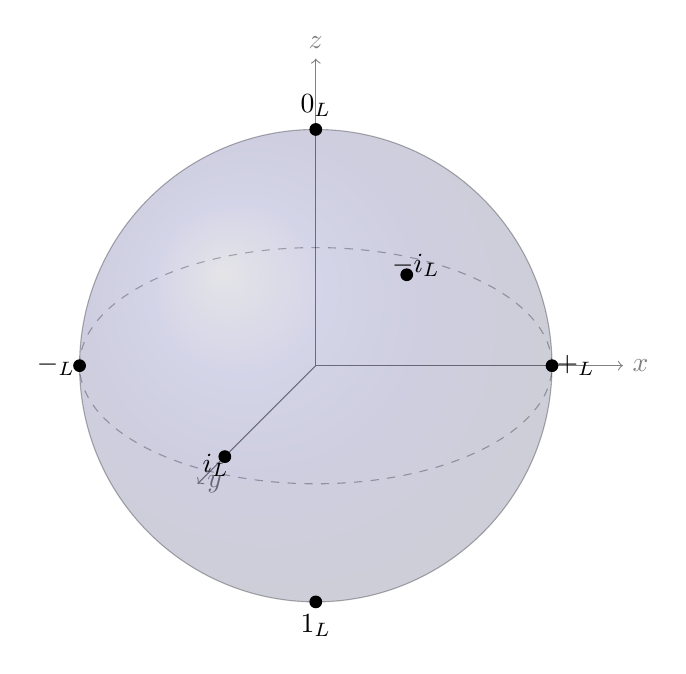
\begin{tikzpicture}[scale=3]
		% --- Ejes ---
		\draw[->, gray] (0,0,0) -- (1.3,0,0) node[anchor=west]{$x$};
		\draw[->, gray] (0,0,0) -- (0,1.3,0) node[anchor=south]{$z$};
		\draw[->, gray] (0,0,0) -- (0,0,1.3) node[anchor=west]{$y$};
		% --- Esfera ---
		\draw[black, opacity=0.3] (0,0) circle (1);
		\draw[dashed, opacity=0.3] (0,0) ellipse (1cm and 0.5cm);
		\fill[ball color=blue, opacity=0.1] (0,0) circle (1);
		% --- Polos (Estados Z) ---
		\node at (0, 1.1) {$\ket{0_L}$};
		\node at (0, -1.1) {$\ket{1_L}$};
		\draw[fill] (0,1) circle (0.7pt);
		\draw[fill] (0,-1) circle (0.7pt);
		% --- Eje X (Estados X) ---
		\node at (1.1, 0, 0) {$\ket{+_L}$};
		\node at (-1.1, 0, 0) {$\ket{-_L}$};
		\draw[fill] (1,0,0) circle (0.7pt);
		\draw[fill] (-1,0,0) circle (0.7pt);
		% --- Eje Y (Estados Y) ---
		\node at (0, 0, 1.1) {$\ket{i_L}$};
		\node at (0, 0, -1.1) {$\ket{-i_L}$};
		\draw[fill] (0,0,1) circle (0.7pt);
		\draw[fill] (0,0,-1) circle (0.7pt);
	\end{tikzpicture}
	\caption{La esfera de Bloch, mostrando la parametrización
		$(\theta, \phi)$ de un estado genérico $\ket{\psi}$ y la ubicación
	de los autoestados de $X_L$, $Y_L$ y $Z_L$.}
	\label{fig:bloch}
\end{figure}
